\section{Animación}

En la animación final, se puede ver como tiene el modificador \textit{Stretch} para simular el aplastamiento y el estiramiento del objeto en movimiento. 

\bigskip

En cuanto al número de plataformas que puede saltar, es un número arbitrario, mayor o igual a 2, por lo que se pueden poner tantas plataformas como se desee, teniendo en cuenta que al aumentar dicho número la velocidad de la animación aumentará, debido a que tendrá que hacer más cosas en el mismo tiempo.

\begin{figure}[H]
   \centering
   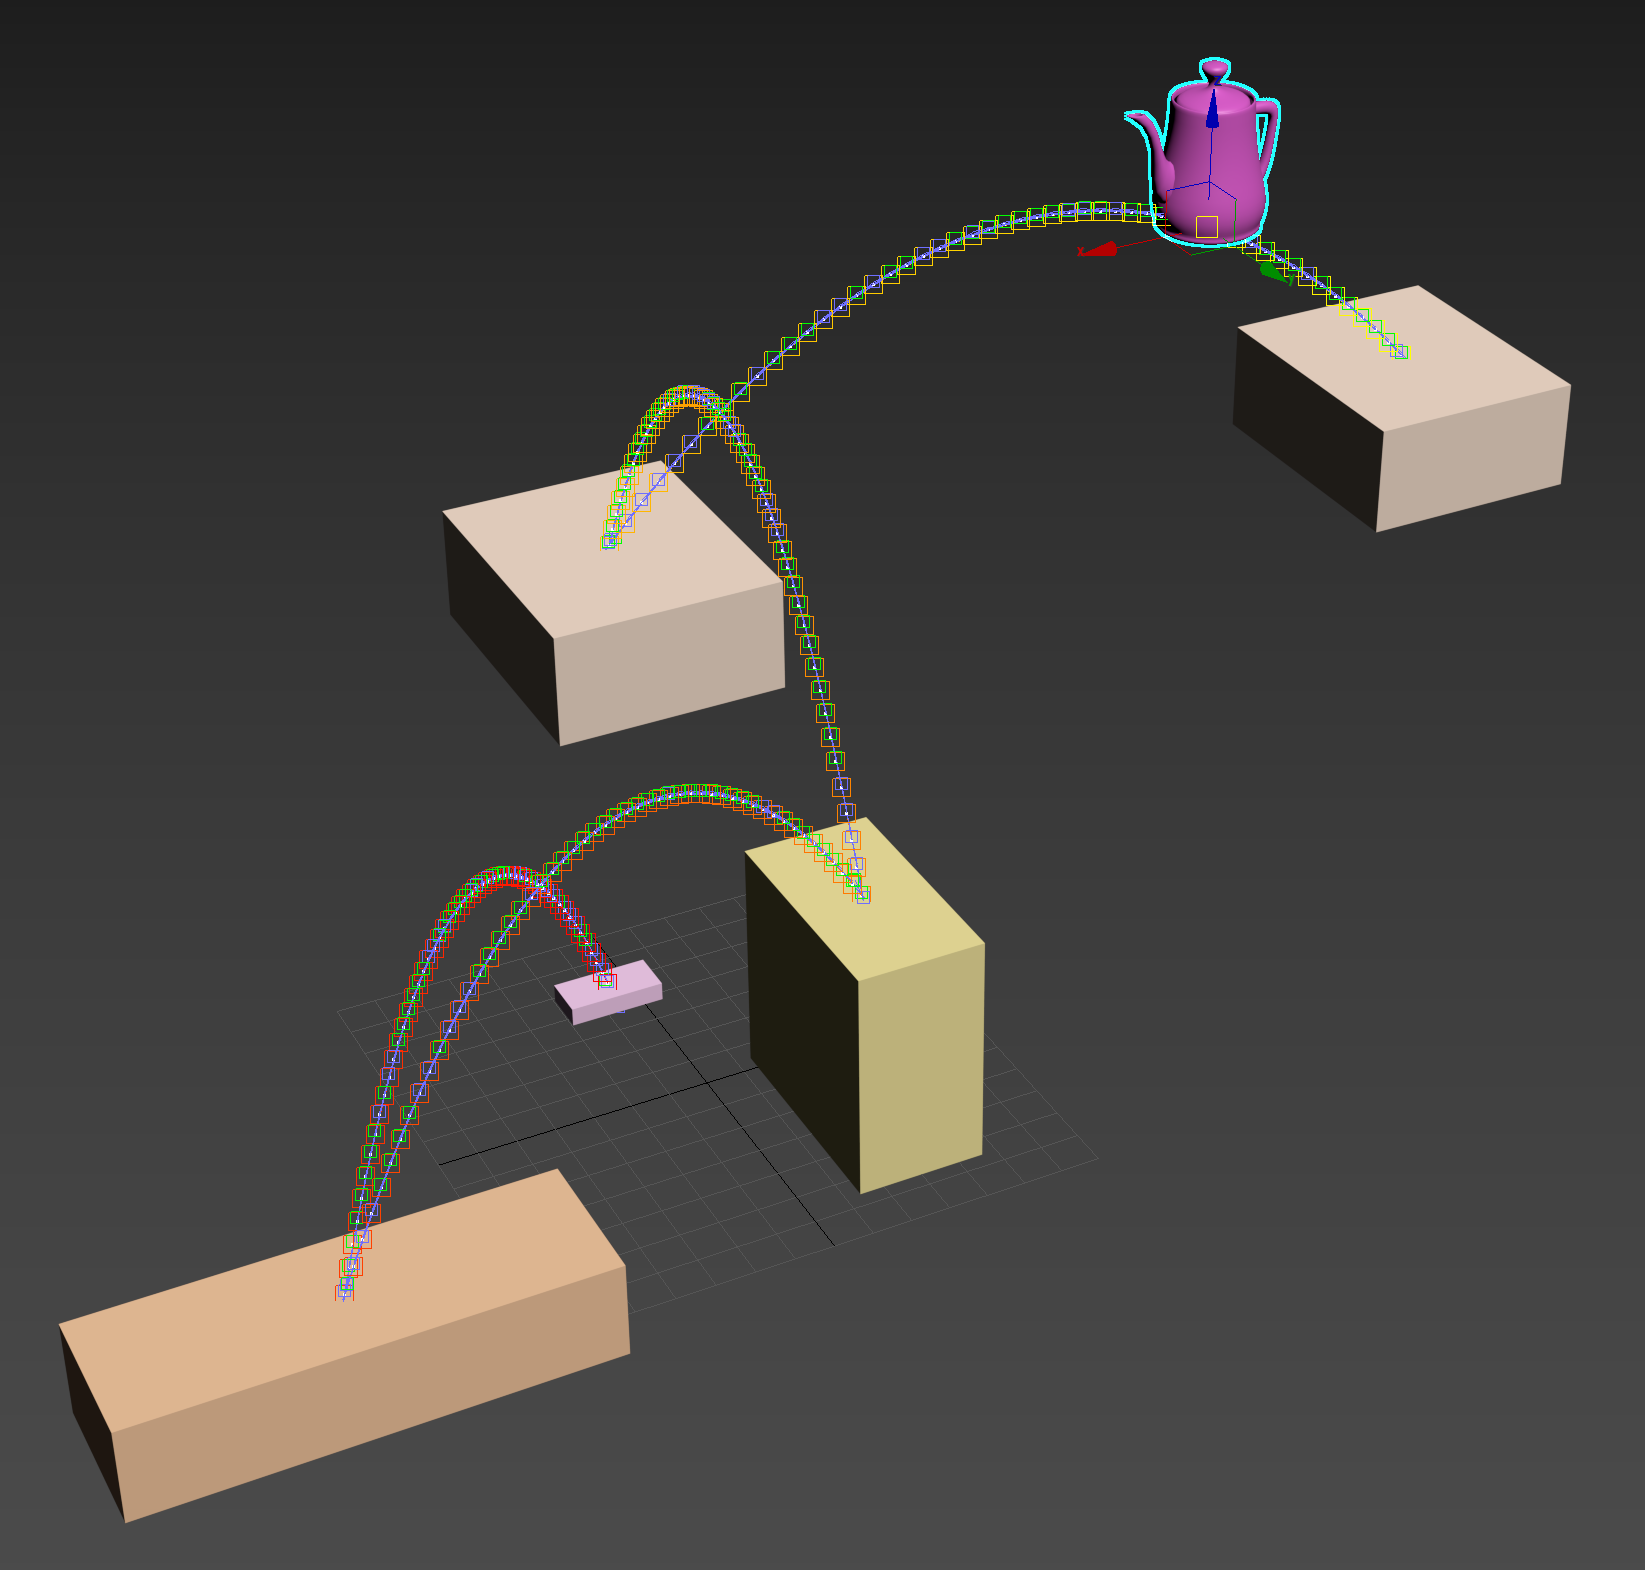
\includegraphics[width=0.62\textwidth]{imagenes/path varios saltos.png}
   \caption{El programa genera todos los saltos necesarios para llegar a todas las plataformas.}
\end{figure}

El punto más alto de cada salto se escoge buscando aquella plataforma que se encuentre más alta y se le suma 120 para que pase por encima de ambas.

\bigskip

Sobre el número de saltos arbitrarios, he necesitado coger las plataformas en pares, de forma que se anime de la plataforma \verb|i| a la plataforma \verb|i+1|, así hasta llegar al final. Cabe destacar que es necesario dividir el número de fotogramas disponibles de manera equitativa, para que los diversos saltos tengan la misma cantidad de tiempo en la animación.

\bigskip

Además, he tenido en cuenta parámetros como que las plataformas no se encuentren en el suelo o se encuentren con un factor de escalado, de forma que la animación resultante siga funcionando.

\bigskip

También he tenido que recortar el \textit{timeline} debido a que si se escogía un valor de inicio distinto de 0, siempre se seguía poniendo ese \textit{keyframe}, haciendo que la animación no fuera correcta hasta llegar al punto de inicio configurado.